\documentclass[11pt, a4paper]{article}

% 页面设计：上(页眉)2.5cm，下(页脚)1.5cm，左3.0cm，右2.4cm
% Added headheight=18pt to accommodate the 15pt header text and prevent fancyhdr errors
\usepackage[top=2.5cm, bottom=1.5cm, left=3.0cm, right=2.4cm, headheight=18pt]{geometry}
\usepackage{fontspec}
\usepackage{graphicx}
\usepackage{fancyhdr}
\usepackage{titlesec} % 用于自定义正文各级标题格式
\usepackage{indentfirst}
\usepackage{float}
\usepackage{zhnumber}
\usepackage{subcaption}
\usepackage{amsmath}
\usepackage{booktabs}
\usepackage{array}
\usepackage{cite}
\let\oldcite\cite
\makeatletter
\renewcommand{\cite}{\@ifnextchar[{\cite@with}{\cite@without}}
\newcommand{\cite@with}[2][]{\textsuperscript{\oldcite[#1]{#2}}}
\newcommand{\cite@without}[1]{\textsuperscript{\oldcite{#1}}}
\makeatother
\usepackage{chngcntr} % 引入计数器宏包
\usepackage{multirow}
\usepackage{etoolbox}
\counterwithin{table}{section} % 让表格的编号跟随 section (节/章) 重新计算
\renewcommand{\thetable}{\arabic{section}-\arabic{table}} % 将默认的点 "." 分隔符改为横线 "-"


\numberwithin{figure}{section}
\renewcommand{\thefigure}{\thesection-\arabic{figure}}
\usepackage[chinese, bidi=basic, provide=*]{babel}
\babelprovide[import, onchar=ids fonts]{chinese}
\babelprovide[import, onchar=ids fonts]{english}

% Set default/Latin font to Sans Serif in the main (rm) slot
\babelfont{rm}{Noto Serif}
\babelfont[chinese]{rm}{Noto Serif CJK SC}
\babelfont{sf}{Noto Sans}
\babelfont[chinese]{sf}{Noto Sans CJK SC}

\usepackage{enumitem}
\setlist[itemize]{label=-,topsep=0pt,itemsep=0pt,parsep=0pt,partopsep=0pt}

% 定义宋体(不加粗)和黑体(不加粗)
\newcommand{\songti}{\rmfamily\mdseries}
\newcommand{\heiti}{\sffamily\mdseries}
\newcommand{\bodyfont}{\songti\fontsize{12pt}{26pt}\selectfont}

%====================
% 标题样式设置
%====================

% 一级标题：居中，宋体加粗，16pt
\titleformat{\section}
  {\centering\songti\bfseries\fontsize{16pt}{26pt}\selectfont}
  {第\zhnumber{\thesection}章}
  {1em}
  {}

% 二级标题：左对齐，宋体加粗，14pt
\titleformat{\subsection}
  {\songti\bfseries\fontsize{14pt}{26pt}\selectfont}
  {\thesubsection}
  {1em}
  {}

% 三级标题：左对齐，宋体加粗，12pt
\titleformat{\subsubsection}
  {\songti\bfseries\fontsize{12pt}{26pt}\selectfont}
  {\thesubsubsection}
  {1em}
  {}

%====================
% 标题与正文间距统一设置
% 参数含义：{左缩进}{标题前距离}{标题后距离}
%====================
\titlespacing{\section}
  {0pt}
  {0pt}
  {0pt}

\titlespacing{\subsection}
  {0pt}
  {0pt}
  {0pt}

\titlespacing{\subsubsection}
  {0pt}
  {0pt}
  {0pt}

%====================
% 封面字段格式
%====================
\newlength{\labwidth}
\newlength{\linewidthcover}
\newlength{\linewidthshort}
\setlength{\labwidth}{3.25cm}
\setlength{\linewidthcover}{11.2cm} % 选题名称的长横线
\setlength{\linewidthshort}{5.5cm}  % 个人信息的短横线

% 专门用于“选题名称”的长横线字段行
\newcommand{\coverlinelong}[2]{%
  {\fontsize{16pt}{30pt}\selectfont % 统一设置该行为 16pt (16号/三号字体)，行距 30pt
   \noindent
   \makebox[\labwidth][c]{\heiti #1}% % 左侧黑体(不加粗)
   \underline{\makebox[\linewidthcover][c]{\songti #2}}% % 右侧宋体(不加粗)
   \par
  }%
}

% 用于其他信息的短横线字段行
\newcommand{\coverline}[2]{%
  {\fontsize{16pt}{30pt}\selectfont % 统一设置该行为 16pt (16号/三号字体)，行距 30pt
   \noindent
   \makebox[\labwidth][c]{\heiti #1}% % 左侧黑体(不加粗)
   \underline{\makebox[\linewidthshort][c]{\songti #2}}% % 右侧宋体(不加粗)
   \par
  }%
}

% 固定 30pt 空行
\newcommand{\coverblankline}{%
  \par\vspace{30pt}%
}

\begin{document}

%====================
% 封面：中期检查报告
%====================
\thispagestyle{empty}

\begin{center}
  \vspace*{0.9cm}

  
\includegraphics[width=7.06cm,height=1.49cm]{image/封面/北京理工大学.png}\par

  \vspace{0.55cm}

  {\songti\bfseries\fontsize{36pt}{43.2pt}\selectfont
   专业学位研究生\\
   中\quad 期\quad 检\quad 查\quad 报\quad 告\par}

  \vspace{1.15cm}

  % 封面填写区：字体不变，行距固定 30pt
  \coverlinelong{选题名称}{面向多智能体系统的高效通信技术研究}
  \coverblankline
  \coverblankline

  \coverline{学\quad\quad 号}{3220241499}
  \coverline{姓\quad\quad 名}{柯逸宸}
  \coverline{导\quad\quad 师}{唐博}
  \coverline{类\quad\quad 别}{电子信息}
  \coverline{领\quad\quad 域}{计算机技术}
  \coverline{培养单位}{珠海校区}

  \coverblankline
  \coverblankline
  \coverblankline

  {\heiti\fontsize{16pt}{30pt}\selectfont 年\quad\quad 月\quad\quad 日}\par
\end{center}

\newpage

%====================
% 正文页眉页脚设置
%====================
\pagestyle{fancy}
\fancyhf{} % 清空默认的页眉和页脚
% 居中页眉[C]：宋体（\songti 已经定义为不加粗），15号字体(15pt)
\fancyhead[C]{\songti\fontsize{15pt}{18pt}\selectfont 北京理工大学专业学位研究生中期检查报告}
% 居中页脚[C]：宋体，五号字体(10.5pt)，显示“第 x 页”
\fancyfoot[C]{\songti\fontsize{10.5pt}{12pt}\selectfont 第\ \thepage\ 页}
\renewcommand{\headrulewidth}{0.4pt} % 页眉下方的横线粗细

%====================
% 目录
%====================
\newpage
{
\songti\mdseries
\fontsize{12pt}{26pt}\selectfont
\renewcommand{\contentsname}{%
  {\songti\bfseries\fontsize{16pt}{26pt}\selectfont 目录}%
}
\setcounter{tocdepth}{2}
\tableofcontents
}
\newpage

%====================
% 正文
%====================
% 正文：宋体，小四号(12pt)，行间距26磅（含图表标题、公式间距等）
\bodyfont
% 让全文基线间距固定为 26pt
\setlength{\baselineskip}{26pt}
% 公式（display math）上下间距按 26pt
\setlength{\abovedisplayskip}{0pt}
\setlength{\belowdisplayskip}{0pt}
\setlength{\abovedisplayshortskip}{0pt}
\setlength{\belowdisplayshortskip}{0pt}
% 插图/表格（浮动体）上下不再额外叠加留白；
% 正文、图题、表题自身均为 12pt / 26pt，避免“26pt 行距 + 26pt 浮动留白”导致实际观感大于 26pt。
\setlength{\intextsep}{0pt}
\setlength{\textfloatsep}{0pt}
\setlength{\floatsep}{0pt}
% 表格内容行高：\fontsize{12pt}{26pt} 已经给出 26pt 行距；
% \arraystretch 只保留 1.0，避免在 26pt 基础上再次放大表格行高。
\renewcommand{\arraystretch}{1.0}
% 表格环境统一继承正文 12pt / 26pt，避免单独表格遗漏设置
\AtBeginEnvironment{table}{\bodyfont}
\AtBeginEnvironment{tabular}{\bodyfont}
% 图/表标题：同正文 12pt/26pt（包含标题多行时的行距）
% 说明：表格标题与表格之间留出半行(13pt)更舒展；图片标题仍不额外加间距
% 取消“图 1-2: ”中的冒号：把 caption 的标签分隔符设为空格
\setlength{\abovecaptionskip}{0pt}
\setlength{\belowcaptionskip}{0pt}
\captionsetup{font={songti,\fontsize{12pt}{26pt}\selectfont},skip=0pt,labelsep=space}
\captionsetup[figure]{font={songti,\fontsize{12pt}{26pt}\selectfont},skip=0pt,labelsep=space}
\captionsetup[table]{font={songti,\fontsize{12pt}{26pt}\selectfont},skip=13pt,labelsep=space}



% --- 第1章 ---
\newpage
\section{引言}
\subsection{研究背景和意义}
\subsubsection{研究背景}
近年来，以Transformer架构为基础的大语言模型（Large Language Models，LLMs）\cite{vaswani2017attention}，如OpenAI的GPT-4系列\cite{ref2}，以及开源生态中的LLaMA系列\cite{ref3,ref4,ref5}、Qwen系列\cite{ref6,ref7,ref8}等，在自然语言理解、逻辑推理与文本生成任务中展现出强大的性能。然而，随着应用场景向高度复杂的现实任务（如软件工程\cite{ref9}、科学计算\cite{ref10}、具身智能探索等\cite{ref11}）拓展，大语言模型的局限性日益凸显\cite{ref12}。

为了突破这一局限，学术界提出了赋予大语言模型自主性的智能体（Agent）概念\cite{ref12}。智能体以大语言模型强大的逻辑推理能力为基础，包括早期的思维链（Chain of Thought，CoT）\cite{ref13}、随后提出的思维一致性（Self-Consistency）\cite{ref14}，以及更复杂的思维树（Tree of Thoughts，ToT）\cite{ref15}和思维图（Graph of Thoughts，GoT）\cite{ref16}。在此基础上，智能体进一步融合了工具调用（Tool Calling/API Use）\cite{ref17,ref18}、环境感知与动态反馈机制，以及长周期复杂任务的拆解与规划能力\cite{ref19}，现已成为当前人工智能领域的核心发展范式\cite{ref20,ref21,ref22}。以ReAct（Reasoning and Acting）\cite{ref23}为代表的方法，将模型的逻辑推理与外部环境执行协同，构建了“思考—行动—观察”的动态闭环，从而显著提升了模型在复杂交互环境中的执行能力\cite{ref24}；同时，Reflexion等基于自然语言反馈的自我修正机制\cite{ref25}，以及Generative Agents、Voyager等\cite{ref26,ref27}引入长时记忆架构，有效克服了大语言模型无状态交互的局限，提升了其可靠性与跨轮次持续学习能力。尽管智能体技术发展迅猛，其能力上限仍受制于三个瓶颈：


\par 1.受限于模型训练数据的日期，其内部权重难以包含最新的知识\cite{ref28}。

\par 2.在上下文窗口限制下，超长输入不仅会带来高昂的计算开销与推理延迟，更易导致关键信息被稀释，引发“迷失在中间（Lost in the Middle）”现象，致使模型丧失对长文本中核心细节的捕捉能力\cite{ref29,ref30}。

\par 3.单智能体受限于单一的推理视角与预设的角色提示词（Prompt），在应对高度复杂、需多学科交叉分析的任务时，极易陷入局部最优的认知局限\cite{ref31}。

为此，学术界与工业界的研究范式正从单体Agent向多智能体系统（Multi-Agent Systems，MAS）演进\cite{ref31,ref32}。MAS通过模拟人类社会的组织与协作机制，引入了明确的角色分工（如程序员、测试员、产品经理的职能划分）与交叉验证辩论体系\cite{ref33,ref34}。大量前沿研究已经初步论证了MAS在复杂场景下的优越性：例如，清华大学提出的ChatDev将软件开发过程建模为瀑布流式的多智能体协作网络，大幅降低了代码漏洞率\cite{ref9}；MetaGPT通过引入标准化操作程序（SOPs），将复杂任务严密拆解为多角色的流水线作业，有效缓解幻觉\cite{ref35}；微软的AutoGen则提供了一种面向对话编程的可定制化多智能体交互模式，支持多个智能体间的灵活组网\cite{ref36}。这些研究充分表明，MAS能够有效突破单智能体的能力天花板，在复杂协同任务中的综合任务成功率、代码通过率与系统鲁棒性均实现了提升。

然而，随着MAS能力的提升，其底层通信机制的瓶颈也暴露出来，成为核心障碍：当前主流的多智能体框架\cite{ref35,ref36}在拓扑维度上多依赖静态的拓扑结构，在语义维度上则普遍采用完全传递的策略。这意味着，每当一个智能体生成内容，其原始输出会被全量且未经筛选地复制给所有相关的下游接收节点。这种密集的交互模式引发了两个问题：

\par 1.通信成本增加：目前模型大多按词元计费。如\ref{fig:communication_bottleneck}所示，一旦智能体数量增多，系统内的消息量就会呈指数级或平方级暴涨，带来巨大的成本压力。
\par 2.关键信息淹没：冗余上下文会导致LLM出现“长上下文注意力衰减”。接收方智能体在处理大量重复和无关的消息时，极易漏掉关键信息，反而拉低了任务的成功率。
\setcounter{figure}{0}

\begin{figure}[H]
  \centering
  \makebox[\textwidth][c]{%
    \subcaptionbox{%
     多智能体系统的token消耗
      \label{fig:communication_bottleneck_left}%
    }[0.45\textwidth]{%
      \includegraphics[width=0.45\textwidth]{\detokenize{image/第一章/图 1‑1-a.png}}%
    }%
    \hspace{0.02\textwidth}%
    \subcaptionbox{%
       不同智能体数量下的输入token
      \label{fig:communication_bottleneck_right}%
    }[0.45\textwidth]{%
      \includegraphics[width=0.45\textwidth]{\detokenize{image/第一章/图 1‑1-b.png}}%
    }%
  }

  \caption{多智能体系统的token消耗对比和不同智能体数量下的输入token变化}
  \label{fig:communication_bottleneck}
\end{figure}

因此，如何减少MAS中高昂通信成本，已成为当前大模型多智能体领域需要解决的问题。针对这一问题，本文提出了一种多智能体系统消息压缩框架，旨在通过对冗余语义信息的过滤与压缩，进而降低多智能体协作过程中的Token消耗，从而为构建低成本的多智能体通信架构提供可靠的解决方案。

\subsubsection{研究意义}
针对当前多智能体系统在通信成本与上下文处理上面临的严峻挑战，本文分析了多智能体系统消息压缩框架具有重要的理论价值与实际意义，体现在以下两个层面：

\par 1.理论意义：
本文从语义信息熵与多智能体通信机制的交叉视角出发，打破了多智能体框架中全量广播的交互范式。通过探索并建立动态、自适应的冗余信息过滤与核心语义保留机制，为解决大语言模型在多轮复杂交互中的“长上下文注意力衰减（Lost in the Middle）”问题提供了新的理论视角。
\par 2.实际意义：
\par（1）降低多智能体系统部署成本：通过对传输消息的压缩，大幅减少了模型推理时的冗余Token消耗。这不仅直接降低了API调用开销，使多智能体系统在工业级、企业级场景中的大规模、低成本部署成为现实。
\par（2）提升多智能体系统的任务成功率：对消息进行压缩为下游智能体提供了关键信息，有效避免了有效信息被海量历史对话淹没。

\subsection{研究基础与目标}
\subsubsection{研究基础}

基于上述背景，在这一部分中，我们将给出大语言模型多智能体系统通信机制中的基础定义，并明确本课题的研究问题。

\textbf{定义1拓扑结构：}表示多智能体系统中各智能体（Agent）节点之间信息交互路径的连接关系。

\textbf{定义2常见通信拓扑类型：}在多智能体协同系统中，根据信息交互路径的组织方式，拓扑结构主要可以划分为以下四种典型范式：

\begin{itemize}[label={·},topsep=0pt,itemsep=0pt,parsep=0pt,partopsep=0pt]
    \item \textbf{完全拓扑（Full Topology）：}指多智能体系统中任意两个智能体节点间均存在双向的信息传输通路。在该拓扑范式下，每个智能体均接收所有其他智能体的输出内容，并将其全量作为历史上下文。
    \item \textbf{层状拓扑（Layered Topology）：}指智能体按层级结构进行划分，当前层的智能体仅接收并处理上一层智能体的输出信息，适用于具有明显阶段划分的复杂任务。
    \item \textbf{链式拓扑（Chain Topology）：}指信息以串行方式依次传递，从初始输入开始，每个智能体顺次处理并将结果单向传递给下一个智能体。
    \item \textbf{星状拓扑（Star Topology）：}指引入中心管理智能体，由其统一负责全局信息的收集、分发与汇总，其余外围智能体与中心节点进行交互。
\end{itemize}

\textbf{定义3语义内容：}指在既定的通信拓扑路径上，智能体之间实际传递的信息内容。在大语言模型多智能体系统中，语义内容通常表现为自然语言文本、结构化提示或中间推理状态。

\textbf{定义4.1单轮内对话：}指多智能体在单个任务对话周期内，通过协同交互共同完成结果输出的交互架构。本研究所探讨的单轮内对话拓扑结构特指完全拓扑，具体如\ref{fig:full_Topology}所示。

\begin{figure}[H]
  \centering
  \includegraphics[width=0.50\textwidth]{\detokenize{image/第一章/图 1‑2：完全通信拓扑.png}}
  \caption{完全拓扑(Full Topology)}
  \label{fig:full_Topology}
\end{figure}
\noindent\textbf{定义4.2多轮间通信：}指多智能体跨对话轮次进行信息传递与历史信息的协作架构。具体表现为在每一轮交互中，每个智能体均接收并利用上一轮所有智能体的输出信息。

\textbf{问题1.1多智能体通信冗余优化：}在多智能体持续协作过程中，随着交互轮次的增加，系统内传递的自然语言上下文会产生严重的语义冗余。如何在约束条件下，寻找最优的过滤机制，从而减少多智能体系统的成本？

围绕上述研究问题，本课题目前已具备以下研究基础：

\par 1.理论与文献基础：已对MetaGPT、AutoGen等主流多智能体协作框架进行了系统性的调研与解构。重点梳理了其底层的交互逻辑、角色分工范式、协同机制以及现有的通信模式。这为本课题重新审视多智能体间的通信瓶颈、进行精确的数学与逻辑建模提供了坚实的理论支撑。
\par 2.技术储备：在通信网络优化的两个核心维度已掌握关键技术，为算法设计提供了直接的方法论支撑。在拓扑结构层面，已掌握图生成、图剪枝及网络拓扑搜索等图论与图学习前沿技术。在语义处理层面，已熟练掌握文本信息压缩相关技术，并深入研究了基于困惑度及轻量化模型辅助的提示词过滤与精简策略。
\par 3.实验环境与资源支持：已具备开展大规模多智能体实验的软硬件条件。目前已获取Qwen、MiniMax\cite{ref60}等主流大型语言模型的API权限及计算资源。

\subsubsection{研究目标}
针对当前多智能体系统（MAS）中由于全量传递所引发的问题，本研究的核心目标是：设计并构建语义驱动的高效多智能体通信架构，在保障或提升任务准确率的前提下，尽可能降低系统的成本。

\subsection{国内外研究现状及分析}

\begin{figure}[H]
  \centering
  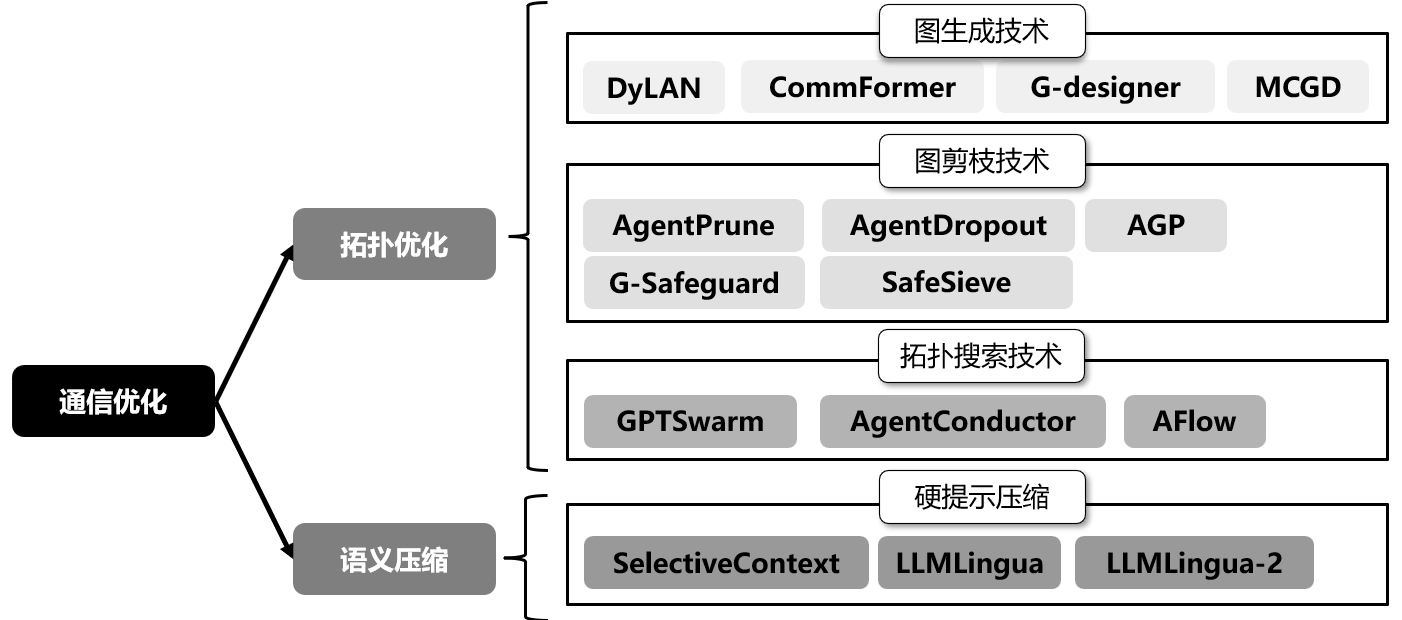
\includegraphics[width=0.65\textwidth]{image/第一章/图 1‑3：多智能体的两条研究路线.png}
  \caption{多智能体的两条研究路线}
  \label{fig:communication_bottleneck}
\end{figure}

为了应对多智能体系统中日益凸显的通信瓶颈，近年来学术界与工业界在通信机制优化方面进行了大量的探索。依据优化策略切入点的不同，现有研究呈现出两条路线：通信拓扑维度的优化（决定信息传播路径，核心目标是减少不必要的通信连接）与语义维度的消息压缩（决定沿路径传递的信息内容，核心目标是减少单条消息内部的冗余）。本章节将分别对两条路线进行系统梳理。

\subsubsection{拓扑维度的优化}

在MAS中，通信拓扑决定了信息的传播广度。其核心优化目标是通过合理规划信息流转的路径，减少不必要的通信交互，从而在拓扑层面降低MAS的词元开销。
早期的MAS框架主要依赖人工预设的静态拓扑（如完全连接、链式/层状、星状或二分图拓扑等\cite{ref9,ref35,ref36,ref37}）。尽管它们在某些结构化任务中提升了效率，但静态设计缺乏对复杂任务的自适应性，且极易导致通信边数随节点数量呈平方级增长，引发词元消耗剧增。
为了克服这一缺陷，当前主流研究方向之一是利用基于图的方法来探索这一问题，即将智能体视为节点、通信链路视为边。近期的相关研究主要可归纳为三大类：图生成、图剪枝与拓扑搜索\cite{ref38}。

\par\textbf{1.图生成技术：}此类方法旨在通过自适应地生成与任务条件相匹配的图，从头开始构建通信拓扑，主要分为以下两种:
\begin{figure}[H]
  \centering
  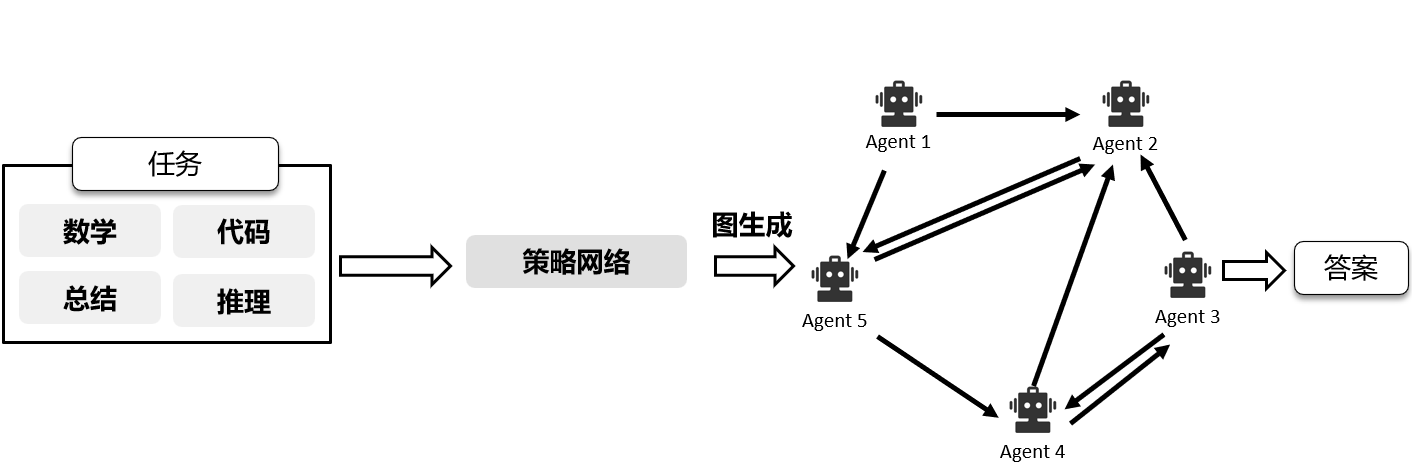
\includegraphics[width=0.65\textwidth]{image/第一章/图1-4：图生成技术.png}
  \caption{图生成技术示意图}
  \label{fig:communication_bottleneck}

\end{figure}

    \par\indent \textbf{询驱动的动态生成：}DyLAN（Dynamic LLM-Agent Network）\cite{ref39}并不预先固定所有智能体之间的通信关系，而是将多智能体协作过程建模为一个随任务推进而变化的前馈式动态网络。其核心机制包括两个阶段：首先在候选智能体集合中进行团队优化，利用Agent Importance Score评估不同智能体在当前任务上的边际贡献；随后在任务求解阶段，根据每一轮中智能体输出的有效性动态选择后续参与通信的节点。DyLAN还引入早停机制，当系统已经形成足够稳定的答案或共识时提前终止多轮交互。因此，它降低成本的方式不是压缩单条消息，而是减少低贡献智能体的参与次数、削减无效讨论轮次，并动态生成更贴合当前查询的通信图。

    \par\indent \textbf{端到端的网络解码：}CommFormer\cite{ref40}将多智能体强化学习中的智能体表示为图节点，将通信信道表示为有向边，并通过可微的图结构学习机制直接优化通信拓扑。其关键做法是对离散边选择进行连续松弛，使邻接矩阵能够参与梯度更新，同时在Transformer结构中引入关系增强注意力，以建模智能体间的依赖关系。训练目标是在合作任务中最大化团队累计回报，同时满足通信稀疏率或通信预算约束。与全连接广播相比，CommFormer只保留对策略协同有显著贡献的通信边，从而在保证任务性能的前提下降低通信开销。

    G-Designer\cite{ref41}面向LLM多智能体系统，将每个智能体的基础模型、角色、状态、工具插件等编码为节点特征，并额外引入任务虚拟节点来表达当前查询需求。随后，它使用变分图自编码器生成面向特定任务的通信图。该方法强调性能、复杂度自适应和鲁棒性三方面目标：简单任务生成较稀疏的拓扑，复杂任务则保留更多协作边。其本质是从任务条件出发解码通信结构，使系统不再依赖人工预设的固定拓扑。

    MCGD\cite{ref42}则更偏向多智能体强化学习中的协调结构建模。它构建包含连续节点属性与离散边属性的稀疏协调图，并利用图扩散模型学习多智能体间的交互模式和动作生成过程。其优化目标是通过扩散式去噪学习恢复有效的协同行为。虽然它不是典型的LLM token通信压缩方法，但其思想同样体现为：只显式建模关键邻居关系，避免全体智能体两两交互带来的结构冗余。


\par\textbf{2.图剪枝技术：}
此类工作通常从密集的拓扑结构（如全连接）开始，旨在将其修剪为稀疏的、适合任务的流水线，同时降低计算成本。

\begin{figure}[H]
  \centering
  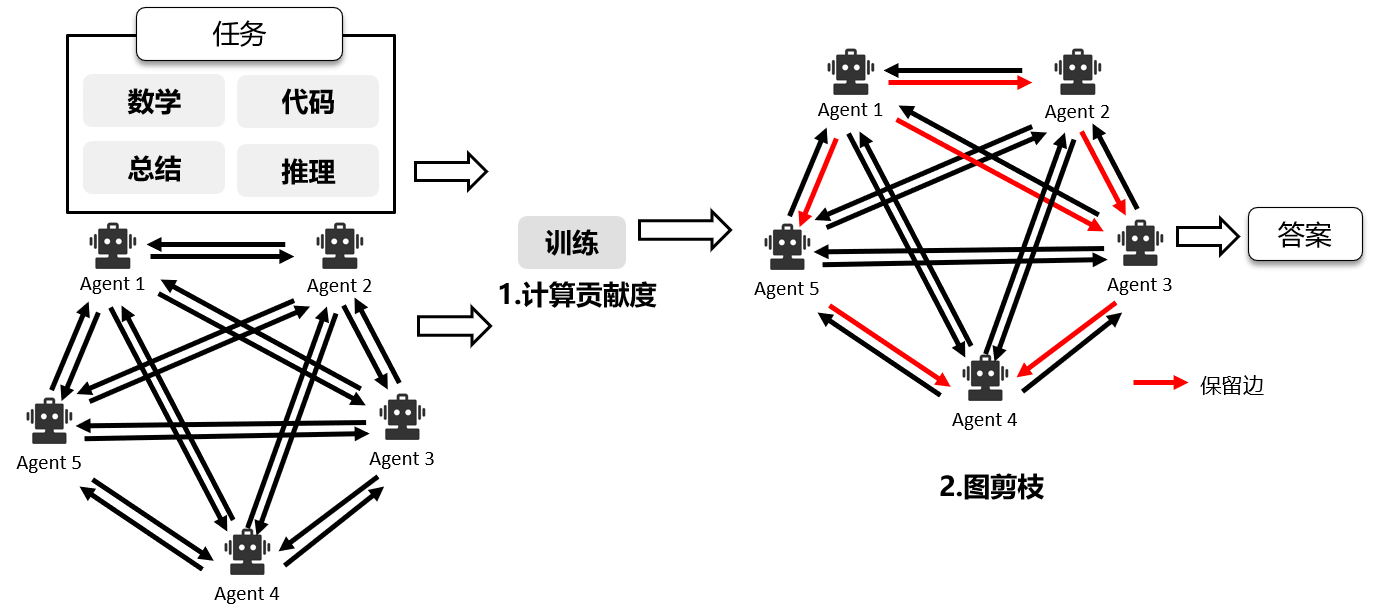
\includegraphics[width=0.65\textwidth]{image/第一章/图1-5：图剪枝技术.png}
  \caption{图剪枝技术示意图}
  \label{fig:communication_bottleneck}
\end{figure}

    \par\indent \textbf{硬剔除与软剪枝：}AgentPrune\cite{ref43}将LLM多智能体系统表示为空间-时间通信图：同一轮智能体之间的信息交换为“空间边”，跨轮历史传递为“时间边”。它为这些边学习可剪枝的图掩码，并通过系统效用评估器判断不同边对任务结果的贡献。由于外部LLM调用和任务评估通常不可微，AgentPrune使用策略梯度近似优化掩码参数。最终，它执行一次性硬剪枝，移除低贡献边，从而同时减少同轮通信和跨轮历史上下文传递。
    AgentDropout\cite{ref44}在边剪枝基础上进一步引入节点丢弃。它首先根据智能体贡献度或加权度识别低价值节点，执行Node Dropout，直接移除部分智能体；随后再通过Edge Dropout剪除剩余智能体之间的低贡献通信边。由于删除一个智能体会同时减少该智能体的输入prompt、输出completion以及后续通信边，因此AgentDropout的成本收益通常比单纯剪边更直接。
    SafeSieve\cite{ref45}采用渐进式软剪枝策略。它首先利用LLM语义评估和角色互补性为通信边初始化重要性分数，再结合历史任务表现不断修正边权。与简单top-k删除不同，SafeSieve使用聚类机制保持核心功能簇的连通性，避免剪枝破坏系统协作结构。因此，它更强调“逐步削弱和删除冗余边”，在保持任务性能和鲁棒性的同时降低token与部署成本。
    AGP（Adaptive Graph Pruning）\cite{ref46}同时进行节点级硬剪枝和边级软剪枝。其训练过程通常分为两步：先采样不同规模的子图，收集高性能通信结构作为监督信号；再训练GNN根据任务表示和智能体嵌入输出节点mask与边权。硬剪枝决定哪些智能体被启用，软剪枝决定启用智能体之间的信息流强度。这样，AGP能针对不同查询生成不同规模的稀疏拓扑，而不是对所有任务使用同一套固定通信结构。
    \par\indent \textbf{基于安全机制的剪枝：}G-Safeguard\cite{ref47}的主要目标是提升LLM多智能体系统的安全性。它构建multi-agent utterance graph，将智能体发言、交互关系和传播路径纳入图神经网络检测框架，用于识别受到prompt injection、memory attack或tool attack影响的异常节点与异常话语。随后系统可以隔离危险智能体或剪断其高风险外发边，阻止恶意信息继续扩散。它的直接收益是安全鲁棒性，通信成本降低更多是拓扑干预带来的副效应。

\par\textbf{3.拓扑搜索技术：}
拓扑搜索通过在智能体算子和通信边构成的庞大图空间中进行探索，以寻优出高效的流水线或通信子图。这类方法通常结合强化学习或网络架构搜索算法。

\begin{figure}[H]
  \centering
  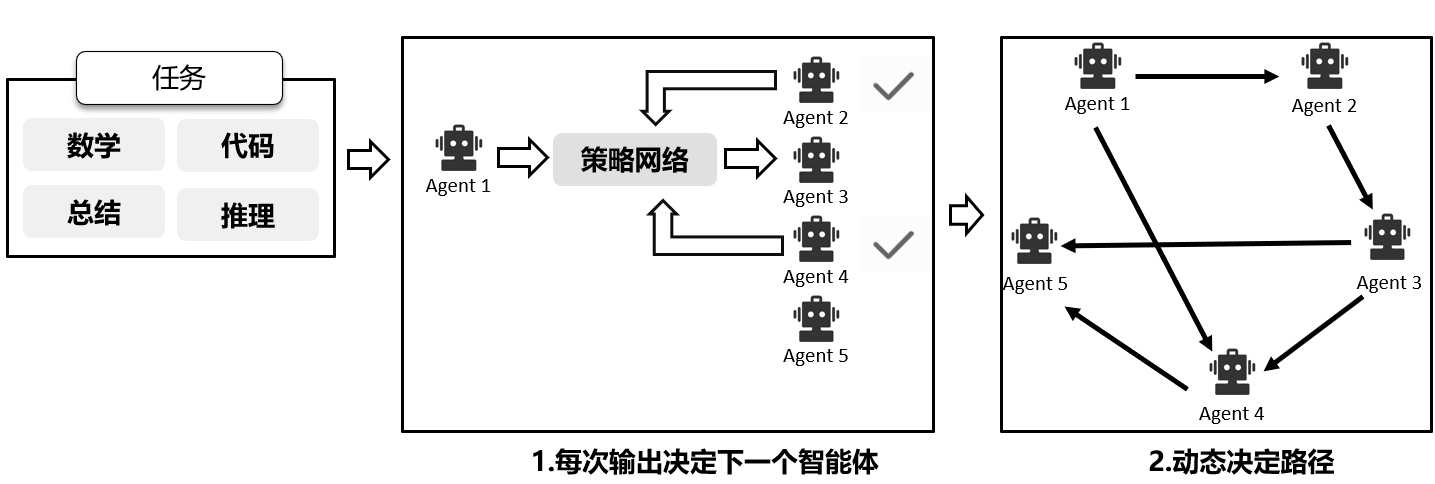
\includegraphics[width=0.65\textwidth]{image/第一章/图1-6：拓扑搜索技术.png}
  \caption{拓扑搜索技术示意图}
  \label{fig:topology_search}
\end{figure}

    \par\indent \textbf{基于强化学习的连续搜索：}GPTSwarm\cite{ref48}将语言智能体系统统一建模为可优化图：节点可以是LLM调用、工具或数据处理函数，边表示信息流。它为候选边分配可学习的采样概率，在无环图空间中采样候选拓扑，并通过REINFORCE等策略梯度方法根据任务效用更新边概率。随着训练推进，低收益边的采样概率趋近于0，高收益边被保留下来，从而形成任务驱动的稀疏通信图。

    AgentConductor\cite{ref49}面向竞赛级代码生成任务，训练一个LLM为每个问题动态生成YAML格式的分层DAG拓扑。图中节点是不同角色的代码智能体，边表示跨层依赖关系，同层节点可并行执行。系统会根据编译、运行和测试反馈多轮调整拓扑。其训练包含监督微调和强化学习，奖励信号同时考虑结构合法性、代码执行结果和难度感知的图密度，因此简单题倾向于生成浅层少边图，复杂题才启用更密集的协作结构。

    \par\indent \textbf{多样化的搜索策略：}AFlow\cite{ref50}将agentic workflow表示为可执行代码中的算子组合与依赖关系。它预定义Generate、Review、Revise、Ensemble、Test、Programmer等工作流算子，并使用蒙特卡洛树搜索在候选工作流空间中探索。每个搜索节点对应一个完整工作流，系统通过验证集执行结果回传分数，逐步扩展更有希望的结构。AFlow不以显式边稀疏正则为核心，而是通过自动搜索找到更短、更有效的工作流程序，从而减少人工设计和冗余调用。

    MASS（Multi-Agent System Search）\cite{ref51}认为多智能体系统的性能同时受prompt和topology影响，因此采用交错优化流程：先优化模块级prompt，再搜索工作流拓扑，最后进行全局prompt优化。其拓扑空间由Aggregate、Reflect、Debate、Summarize、Tool-use等方式构成。MASS会评估不同模块相对于单智能体基线的贡献，对低收益或负收益模块进行影响力剪枝，再在剩余空间中采样和验证候选拓扑。

    MaAS（Multi-agent Architecture Search via Agentic Supernet）\cite{ref52}提出“智能体超网”思想，将多智能体架构表示为可按查询采样的层级子网。控制器根据query embedding和上一层已选算子，逐层选择Generate、SelfRefine、Programmer、Ensemble等候选算子。其训练使用策略梯度式目标，效用函数通常同时考虑任务得分和调用成本。推理时，每个查询只激活超网中的少量算子路径，并可结合早停机制降低token和调用开销。

    DynaSwarm\cite{ref53}则在GPTSwarm式参数化通信图基础上进一步引入样本级动态选择。它先通过Actor-Critic学习多个高性能候选图，再训练graph selector根据输入样本选择最合适的拓扑。使得系统不再依赖一个全局静态最优图，而是针对不同任务实例路由到不同稀疏候选结构，在保持较低选择延迟的同时提升拓扑适配性。


\subsubsection{语义维度的压缩}
除了在通信拓扑层面减少冗余交互外，在语义维度直接对智能体传递的上下文消息进行压缩，是降低大型语言模型（LLMs）推理成本、提升内存利用率的另一项重要手段。与拓扑优化关注“哪些智能体之间需要通信”不同，语义压缩更关注“沿通信链路传递什么内容”，其核心思想是在尽量保持任务相关语义不丢失的前提下，减少上下文中的冗余词元、重复表述和低价值信息。在实现这一目标的诸多策略中，硬提示词压缩技术（Hard Prompt Methods）作为一种无需修改模型底层架构、能够直接适配黑盒LLM接口的实用方案，受到了学术界和工业界的广泛关注。本节将重点探讨此类技术。

硬提示词压缩旨在通过对原始文本进行修改，生成人类可读的、更为精简的自然语言序列。与软提示压缩将上下文映射为不可读的连续向量不同，硬提示词压缩保留了自然语言形式，因此更便于人工检查、跨模型迁移以及在多智能体通信场景中复用。根据压缩机制的不同，主流研究主要可划分为以下两个方向\cite{ref54}：

\begin{figure}[H]
  \centering
  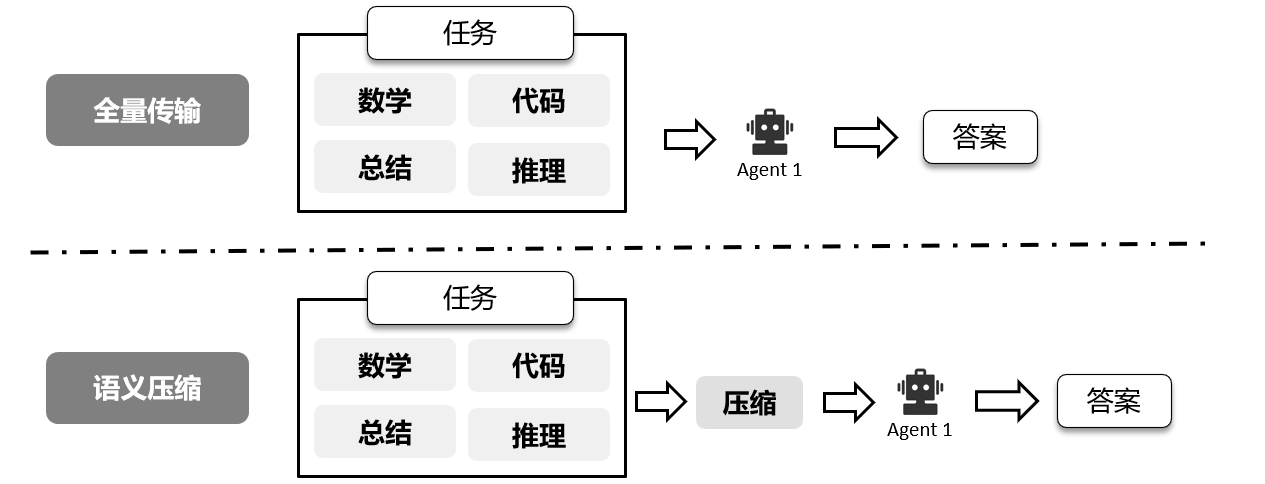
\includegraphics[width=0.65\textwidth]{image/第一章/图1-7：压缩示意图.png}
  \caption{压缩示意图}
  \label{fig:communication_bottleneck}
\end{figure}

    \par\textbf{1.基于过滤与剪枝(Filtering)：}此类方法通过评估词元、短语或句子的重要性，剔除冗余和低信息量的部分，并在保持原文顺序的基础上生成压缩后的上下文。早期代表性工作SelectiveContext\cite{ref55}利用较小规模的因果语言模型计算词元的自信息或困惑度，将低自信息内容视为更容易由上下文预测、因而冗余度更高的部分，再按照词元、短语或句子粒度进行过滤。该方法无需额外训练，能够直接应用于黑盒LLM，但由于其重要性评估主要依赖语言统计特征，可能误删对特定任务有用但语言上并不突出的信息。LLMLingua\cite{ref56}进一步提出粗到细的压缩框架，首先通过预算控制器在指令、示例和问题等不同提示词组成部分之间分配压缩率，再利用小模型估计词元困惑度或信息熵，逐步保留高信息量词元。相比简单过滤，LLMLingua考虑了提示词内部不同模块的重要性差异，并通过迭代式压缩缓解局部删除造成的上下文断裂问题，因此能够在较高压缩率下保持较好的下游任务性能。

    后续的LLMLingua-2\cite{ref57}则引入了数据蒸馏机制，将压缩任务从基于困惑度的无监督筛选转化为词元级二分类任务。具体而言，该方法先利用强模型生成抽取式压缩结果，再通过自动对齐为原始文本中的词元标注“保留”或“删除”标签，并训练轻量级双向编码器预测每个词元的重要性。推理时，模型按照保留概率选择满足压缩预算的词元，并保持其原始顺序。由于双向编码器能够同时利用左右上下文，LLMLingua-2在压缩速度、忠实度和跨任务泛化方面均优于单纯依赖困惑度的方法。进一步地，TACO-RL\cite{ref58}将强化学习引入过滤式压缩过程，将每个词元的保留或删除视为动作，并根据下游任务表现给予奖励。例如，在问答任务中可依据答案F1值评估压缩效果，在摘要任务中可依据生成文本与参考文本的相似度计算奖励。通过这种方式，TACO-RL能够根据具体任务目标动态调整剪枝策略，使压缩器更倾向于保留与当前查询或任务评价指标直接相关的信息，从而弥补任务无关过滤方法在语义选择上的不足。

    \par\textbf{2.基于释义与重写(Paraphrasing)：}与简单的删除词元不同，此类方法利用语言模型强大的生成与概括能力，主动将冗长的上下文重写为更紧凑的自然语言表达。其核心优势在于能够跨越句子边界进行信息重组，将分散在原文不同位置的关键信息合并为更短的表述，从而避免纯过滤方法可能造成的语义割裂或可读性下降。例如Nano-Capsulator框架\cite{ref59}不再直接从原始提示词中选择词元，而是训练一个生成式压缩模型，将长提示词封装为更短的Capsule Prompt。该模型在训练过程中同时考虑语义保持和下游任务效用：一方面要求压缩后的自然语言表示尽可能保留原始提示词的核心含义，另一方面又通过目标LLM在相关任务上的输出表现约束压缩结果，使其不仅短，而且仍然能够有效引导模型完成任务。

    与过滤式方法相比，基于释义与重写的压缩能够生成更加流畅、连贯且人类可读的压缩文本，尤其适合处理包含重复解释、长链式推理示例或多轮对话历史的上下文。在多智能体系统中，这类方法可用于将某一智能体的长篇推理过程、观察记录或工具调用结果重写为面向后续智能体的短摘要，从而减少跨智能体传递的词元数量。然而，这类方法也存在一定风险：由于压缩过程依赖生成模型，可能出现关键信息遗漏、语义偏移甚至幻觉。因此，在高精度任务中，重写式压缩通常需要结合任务反馈、事实一致性检测或保守的压缩率设置，以在压缩效率与语义可靠性之间取得平衡。

% --- 第2章 ---
\newpage
\section{研究内容}

在这一章节中，我们将详细阐述如何将通信优化嵌入多智能体系统任务执行流程，并解析各个功能模块的具体设计。

\subsection{研究方案概述}

在这一章节中，我们将描述当前多智能体执行的流程，并给出消息压缩框架的初步设计。

\subsubsection{多智能体系统任务执行流程}

多智能体系统通过角色分工与协作推理来完成目标。如图\ref{fig:mas_workflow}所示，其标准任务执行流程主要包含以下四个核心环节：

\begin{enumerate}[
    topsep=0pt,
    itemsep=0pt,
    parsep=0pt,
    partopsep=0pt,
    leftmargin=0em,
    itemindent=2em,
    label=\arabic*.
]
    \item \textbf{任务输入：}接收并标准化外部任务，为智能体构建结构化的上下文环境。
    \item \textbf{协作推理：}依托预设的通信拓扑，各智能体结合自身角色与前驱节点的历史信息进行多轮次推理，并持续传递中间结果。
    \item \textbf{结果聚合：}采用投票或共识决策机制，对各智能体的候选答案进行汇总，输出最终可靠结果。
    \item \textbf{性能评测：}系统性评估模型在任务准确率及通信成本（如词元消耗、推理延迟）上的综合表现。
\end{enumerate}

\begin{figure}[htbp]
    \centering
    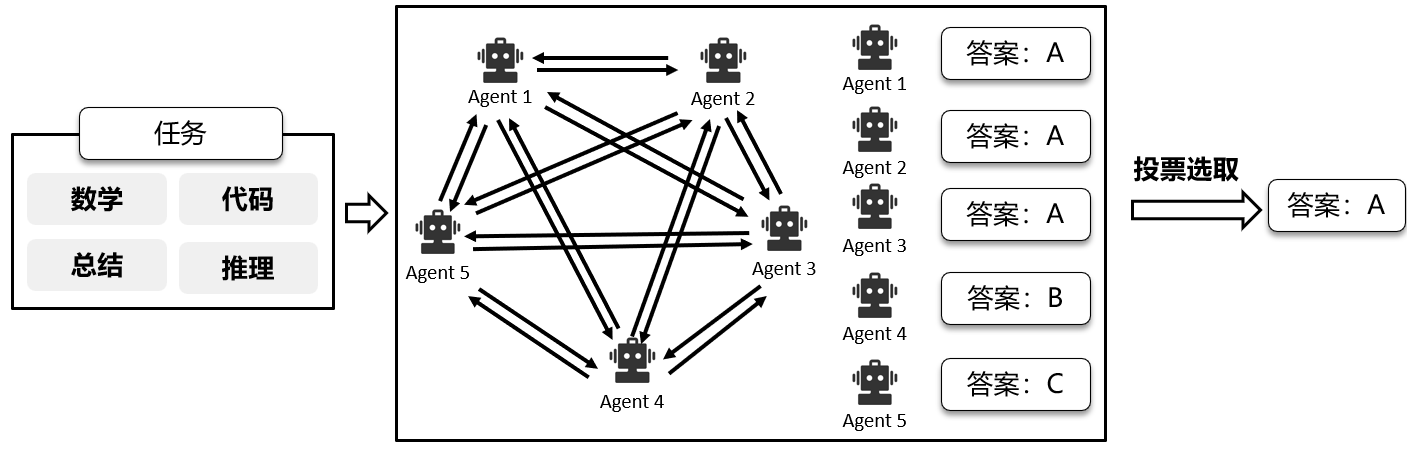
\includegraphics[width=0.85\linewidth]{image/第二章/图 2‑1 多智能体系统标准任务执行流程示意图.png}
    \caption{多智能体系统标准任务执行流程示意图}
    \label{fig:mas_workflow}
\end{figure}

\subsubsection{消息压缩框架执行流程}

为解决多智能体协作中的信息冗余问题，本课题在智能体与智能体之间的通信中引入了\textbf{消息压缩框架}。该框架从角色、节点和时序三个维度对通信内容进行压缩。

具体执行流程包含以下三个核心步骤：

\begin{enumerate}[
    topsep=0pt,
    itemsep=0pt,
    parsep=0pt,
    partopsep=0pt,
    leftmargin=0em,
    itemindent=2em,
    label=\arabic*.
]
    \item \textbf{角色感知压缩：}针对接收方信息需求的不对称性，根据下游角色的具体职责，过滤前驱智能体消息中的无关推理内容，从而使下游智能体能够获得与自身任务更相关的信息。
    \item \textbf{节点感知聚合：}针对多个前驱节点可能产生相似推理内容的问题，将不同节点传来的相似推理过程进行去重，避免相同观点在下游智能体上下文中重复出现，从而减少冗余消息传递。
    \item \textbf{分歧感知压缩：}针对多轮对话记录过长的问题，通过提取历史轮次中的共识与分歧内容，压缩上一轮次传递的信息，并保留有效信息供本轮智能体参考。
\end{enumerate}

\begin{figure}[htbp]
    \centering
    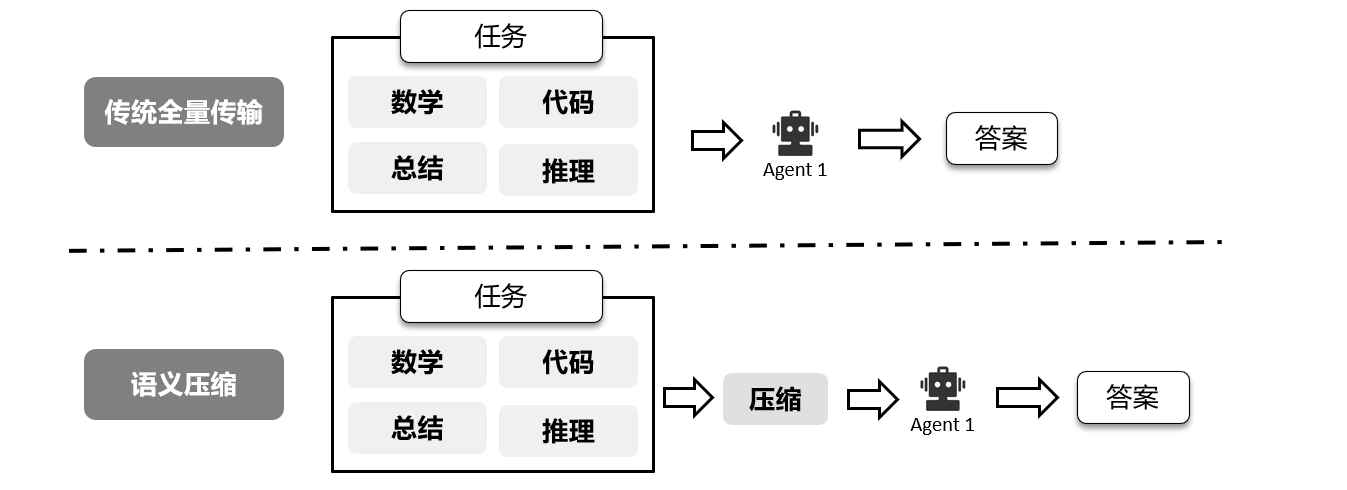
\includegraphics[width=0.85\linewidth]{image/第二章/图2-2 消息压缩框架.png}
    \caption{消息压缩框架}
    \label{fig:message_compression_framework}
\end{figure}


\subsection{功能模块设计}

本节介绍消息压缩框架的三个核心模块：角色感知消息压缩、节点感知消息聚合和时序答案一致性摘要。三者分别处理多智能体通信中的三类冗余：第一类是发送方推理内容与接收方角色无关，第二类是多个前驱智能体给出了相似推理，第三类是跨轮历史持续累积导致上下文过长。为避免符号堆叠，本文仅保留必要定义，并重点说明各模块的输入、处理逻辑和输出结果。

设多智能体系统的通信图为$G=(V,E)$。在第$t$轮中，发送方智能体$u$传递给接收方智能体$v$的消息表示为
$$
m_{u\rightarrow v}^{(t)}=(r_u^{(t)},a_u^{(t)}),
$$
其中$r_u^{(t)}$表示推理内容，$a_u^{(t)}$表示最终答案。本文的压缩操作主要作用于推理内容$r_u^{(t)}$，原则上不直接改写答案字段，从而避免压缩过程破坏最终判断。

\subsubsection{角色感知压缩模块}

角色感知压缩模块解决的是“消息是否适合当前接收方”的问题。在多智能体系统中，不同智能体承担的职责不同。例如，负责规划的智能体更需要任务拆解和约束信息，负责验证的智能体更关注候选答案、错误风险和反例。如果发送方的完整推理被直接转发给所有下游节点，接收方会同时看到大量与自身职责无关的内容，既增加token成本，也容易稀释真正有用的信息。

该模块的处理流程分为三步。首先，将发送方的推理文本按句子切分，得到若干候选推理片段。其次，将每个句子与接收方角色描述进行语义匹配，匹配分数由文本向量的余弦相似度给出：
$$
\operatorname{sim}(s,d_v)=\cos(\phi(s),\phi(d_v)),
$$
其中$s$表示候选句子，$d_v$表示接收方角色描述，$\phi(\cdot)$表示文本编码函数。最后，系统根据同一条消息内部的相似度分布自动确定保留阈值，只保留与接收方角色更相关的句子；若保留文本仍超过角色预算，则按原始顺序截断到预算范围内。

该模块的输出仍然是一条结构化消息：推理字段被替换为筛选后的短文本，答案字段保持不变。这样做的好处是，接收方能够获得更贴近自身职责的上下文，同时不会因为压缩推理过程而丢失发送方给出的最终答案。

\subsubsection{节点感知聚合模块}

节点感知聚合模块解决的是“多个前驱消息之间是否重复”的问题。对于同一个接收方节点，多个上游智能体可能从不同角度得出相近结论，也可能在推理过程中反复陈述同一事实。如果将这些内容直接拼接，下游节点会接收到大量重复表达，导致上下文变长，但信息增量有限。

该模块会先收集接收方节点所有前驱智能体的压缩后推理句子，并为每个句子保留来源角色标签。随后，系统按照句子出现顺序逐一检查候选内容：若当前句子与已保留句子的语义相似度高于冗余阈值，则认为它提供的信息已经被覆盖，不再重复加入；若相似度低于阈值，则将其作为新的有效信息保留。本文实现中，冗余判定阈值取$0.70$，用于在“去重”和“保留多样观点”之间取得平衡。

聚合后的推理内容由若干带角色标签的句子组成。角色标签的作用是保留信息来源，使下游智能体不仅知道“有哪些观点被保留”，也能知道“这些观点来自哪个角色”。对于多个前驱节点给出的答案，模块采用简单投票生成聚合答案；若出现票数接近或无法明确多数的情况，则保留多个候选答案及其来源，交由后续节点继续判断。

通过该模块，系统不再把多个前驱消息拼接，而是先做跨节点去重和来源标注。这样既能减少重复token，也能提高下游上下文的信息密度。

\subsubsection{分歧感知压缩模块}

分歧感知压缩模块解决的是“跨轮历史如何保留”的问题。多智能体协作通常需要多轮执行，如果每一轮都完整保存所有智能体的推理和答案，历史记忆会快速膨胀。过长的历史不仅增加推理成本，还可能使模型在后续轮次中难以抓住当前最关键的共识和分歧。

该模块在每一轮协作结束后运行。系统首先收集本轮所有智能体的答案，并对答案文本进行规则化处理，例如去除多余空格、统一大小写、去掉常见答案前缀和标点。经过规则化后，表达相同含义的答案会被归入同一个答案组。基于答案组数量，系统生成两类摘要。

当所有智能体的答案归入同一组时，说明本轮协作已经形成共识。此时摘要只保留共识答案，以及最能代表该结论的简短理由。代表理由通常来自推理内容较完整的智能体，并只保留核心句子，避免把完整推理链再次写入历史。

当答案被分成多个组时，说明智能体之间仍存在分歧。此时摘要会记录每个候选答案、支持该答案的智能体数量，以及对应的简短理由。这样，下一轮智能体能够直接看到当前争议点，而不需要重新阅读上一轮所有冗长输出。

最终生成的摘要会写入各智能体的历史记忆，作为下一轮推理的压缩上下文。该模块只依赖规则化文本处理、答案分组和简短摘要模板，不额外调用大语言模型，因此能够在控制成本的同时保留跨轮协作中最重要的信息。

% --- 第3章 ---
\newpage

\section{实验与分析}
\subsection{实验设置}
目前，消息压缩框架实现已完成，我们在一些数据集中进行了实验，在本章节中将会展示已经完成的实验结果，并给出对应结果的分析。

\subsubsection{数据集}
为全面客观地评估模型能力，本文从多智能体系统领域广泛认可的6个数据集，涵盖综合知识、数学推理和代码生成三个核心能力维度。具体任务特征与选取依据如表3-1所示。


\vspace{26pt}
\begin{table}[H]
    \centering
    {
        \fontsize{12pt}{26pt}\selectfont
        % 使用 p{宽度} 让第二、第三列允许自动折行。您可以根据页面余白微调这里的 3.5cm 和 6.5cm
        \begin{tabular}{|c|p{3.5cm}|p{6.5cm}|c|}
            \hline
            任务类型 & 数据集名称 & 描述 & 样本数量\\
            \hline
            综合知识 & MMLU\cite{ref61} & 涵盖57个不同学科的综合性基准 & 153 \\
            \hline
            % 使用 \multirow 进行跨行合并，数字 4 代表跨 4 行
            \multirow{4}{*}{数学推理} & GSM8K\cite{ref62} & 小学数学应用题数据集 & 1319 \\
            \cline{2-4} % 画一条只贯穿第2到第4列的横线，避开合并的第1列
             & AQuA\cite{ref63}& 复杂的代数应用题 & 254 \\
            \cline{2-4}
             & MultiArith\cite{ref64} & 多步算术运算 & 600 \\
            \cline{2-4}
             & SVAMP\cite{ref65} & 语义和扰动生成的数学题 & 1000 \\
            \hline
            代码生成 & HumanEval\cite{ref66} & 生成完整Python代码 & 164 \\
            \hline
        \end{tabular}
    }
    \caption{实验评测数据集概览}
    \label{tab:dataset_overview}
\end{table}

\subsubsection{基座模型}
为了保证实验结论的客观性与普适性，本文选取了两个主流大语言模型作为多智能体的基座。这两个模型在API调用成本存在显著差异。具体模型计费标准如表3-2所示。
\vspace{26pt}
\begin{table}[H]
    \centering
    {
        \fontsize{12pt}{26pt}\selectfont
        \begin{tabular}{|l|c|c|}
            \hline
            模型名称 & 输入价格（千tokens） & 输出价格（千tokens）\\
            \hline
            Qwen2.5-14B-Instruct  & ¥0.0007 & ¥0.0007 \\
            \hline
            Qwen3-14B  & ¥0.0005 & ¥0.0020 \\
            \hline
            MinMax-M3  & ¥0.0021 & ¥0.0084 \\
            \hline

        \end{tabular}
    }
    \caption{API调用单价对比表}
    \label{tab:base_model_api_price}
\end{table}

Qwen2.5-14B-Instruct：作为24年开源指令模型的代表，其在通用问答、指令遵循与文本生成等任务中表现出较高的稳定性。本研究将其设为基础对照组，旨在与 Qwen3-14B 形成严格的控制变量（参数量级一致）。通过引入该对照组，重点考察在缺乏新一代推理与指令优化机制的前提下，消息压缩策略对任务生成质量、词元（Token）消耗及调用成本的具体影响。

Qwen3-14B：作为中等规模参数开源模型的代表，该模型在推理效率、部署成本与基础性能之间实现了较优的平衡。结合表 3-1 数据可知，其 API 调用成本相对低廉。选取该模型旨在探究消息压缩策略在低成本、常规算力约束下，对实际任务效能及经济成本的优化潜力。

MinMax-M3：引入该闭源商业模型旨在拓展实验基座的架构多样性，并构建高成本模型对照场景。鉴于其 API 调用费率显著较高（输入与输出单价约为 Qwen3-14B 的 4 倍以上），在处理长文本任务时极易产生高昂的边际成本。选取该模型旨在验证消息压缩策略在面对高资源消耗型商业大模型时，能否有效降低计算冗余并实现显著的成本缩减。

在所有实验中，均采用相同的系统提示词、智能体数量、超参数以及数据集划分，以确保实验结果的可比性。


\subsubsection{对比方法}实验构建了三种通信拓扑作为对比。首先是完全拓扑基线，上游智能体生成的原始输出直接、完整地透传给下游智能体，不进行任何截断，从而保留了完整的上下文内容，其代表了系统通信开销的上限及任务基础性能的对照标准。其次是AgentPrune方法基线，作为当前多智能体系统拓扑优化的代表性方法，该基线对智能体间的通信边进行剪枝。最后是本文方法，即引入本文设计的消息压缩模块，在智能体交互前对冗长的推理和弱相关背景进行压缩，仅精准保留关键信息。

\subsubsection{评估指标}本文主要从任务完成质量与通信成本两个维度，选取了以下两项核心评价指标：
\par \textbf{准确率 (Accuracy,)：}衡量模型完成任务的有效性。针对MMLU及四项数学推理数据集（GSM8K、AQuA、MultiArith、SVAMP），提取模型最终输出的答案与标准答案进行精确匹配以计算正确率；对于HumanEval代码生成数据集，则以测试用例的通过率（Pass@1）作为准确率进行评估。
\par \textbf{词元花费 (Token Cost)：}衡量多智能体通信过程中的经济开销。具体统计系统在完成单次完整任务时，所消耗token的价格。


\subsection{实验结果和分析}

本阶段实验在MMLU、GSM8K、AQuA、MultiArith、SVAMP和HumanEval六个数据集上展开，覆盖通用知识理解、数学推理、多项选择推理和代码生成等不同任务类型。实验对比了Direct、Fullconnect、Agentprune和本文方法。

为保证总体结果统计的可解释性，本文在主实验中选取MiniMax-M3、Qwen3-14B和Qwen2.5-14B-Instruct作为主要分析模型，并按模型分别计算其在可用数据集上的平均表现。其中MiniMax-M3和Qwen3-14B覆盖MMLU、GSM8K、AQuA、MultiArith、SVAMP和HumanEval六个数据集；Qwen2.5-14B-Instruct目前覆盖除GSM8K外的五个数据集。总体实验不将所有模型和数据集混合为单一平均值，而是分别展示三个模型下不同方法的平均表现，以避免模型覆盖范围不同带来的统计偏差。

\subsubsection{推理性能分析}

\begin{figure}[H]
    \centering
    \includegraphics[width=0.82\linewidth]{\detokenize{image/第三章/figures/summary/fig1_model_average_accuracy_bars.png}}
    \caption{六个数据集在不同模型下的平均准确率对比}
    \label{fig:summary_model_accuracy}
\end{figure}

图\ref{fig:summary_model_accuracy}展示了三个主要模型在不同方法下的跨数据集平均准确率。整体来看，本文方法在Qwen3-14B和Qwen2.5-14B-Instruct上均取得最高平均准确率，在MiniMax-M3上与Direct方法基本持平，同时高于Fullconnect和Agentprune。这说明本文方法在不同模型能力水平下均具有较好的稳定性，尤其在中小规模模型上能够带来更明显的性能收益。

具体而言，在Qwen3-14B上，本文方法的平均准确率达到93.10\%，高于Direct的92.80\%、Fullconnect的92.53\%和Agentprune的91.20\%。在Qwen2.5-14B-Instruct上，本文方法的平均准确率为88.46\%，高于Direct的86.62\%、Fullconnect的88.08\%和Agentprune的87.42\%。在MiniMax-M3上，Direct方法的平均准确率为93.72\%，本文方法为93.66\%，二者差距仅为0.06个百分点，基本处于同一水平；同时，本文方法仍高于Fullconnect和Agentprune。

为了避免总体平均掩盖不同任务类型的差异，下面进一步按数据集展开分析。总体上，本文方法在MMLU、GSM8K、MultiArith和SVAMP上表现较强，在AQuA和HumanEval上则呈现出更明显的任务依赖性，说明消息级协作更适合知识理解和数学推理类任务，而在多项选择干扰项较强或代码生成需要执行反馈的任务中仍有改进空间。


\begin{figure}[H]
    \centering
    \makebox[\textwidth][c]{%
        \subcaptionbox{MMLU准确率
        \label{fig:mmlu_accuracy_panel}}[0.46\textwidth]{%
            \includegraphics[width=\linewidth]{\detokenize{image/第三章/figures/mmlu/fig2_accuracy_bars.png}}%
        }%
        \hspace{0.02\textwidth}%
        \subcaptionbox{GSM8K准确率
        \label{fig:gsm8k_accuracy_panel}}[0.46\textwidth]{%
            \includegraphics[width=\linewidth]{\detokenize{image/第三章/figures/gsm8k/fig2_accuracy_bars.png}}%
        }%
    }
    \vspace{0.5em}

    \makebox[\textwidth][c]{%
        \subcaptionbox{AQuA准确率
        \label{fig:aqua_accuracy_panel}}[0.46\textwidth]{%
            \includegraphics[width=\linewidth]{\detokenize{image/第三章/figures/aqua/fig2_accuracy_bars.png}}%
        }%
        \hspace{0.02\textwidth}%
        \subcaptionbox{MultiArith准确率
        \label{fig:multiarith_accuracy_panel}}[0.46\textwidth]{%
            \includegraphics[width=\linewidth]{\detokenize{image/第三章/figures/multiarith/fig2_accuracy_bars.png}}%
        }%
    }
    \vspace{0.5em}

    \makebox[\textwidth][c]{%
        \subcaptionbox{SVAMP准确率
        \label{fig:svamp_accuracy_panel}}[0.46\textwidth]{%
            \includegraphics[width=\linewidth]{\detokenize{image/第三章/figures/svamp/fig2_accuracy_bars.png}}%
        }%
        \hspace{0.02\textwidth}%
        \subcaptionbox{HumanEval准确率
        \label{fig:humaneval_accuracy_panel}}[0.46\textwidth]{%
            \includegraphics[width=\linewidth]{\detokenize{image/第三章/figures/humaneval/fig2_accuracy_bars.png}}%
        }%
    }
    \caption{各数据集上不同模型与方法的准确率对比}
    \label{fig:dataset_accuracy_panels}
\end{figure}


\noindent\textbf{MMLU}在MMLU数据集上，本文方法整体表现较为稳定。在主分析的三个模型中，本文方法的平均准确率为87.10\%，高于Direct的83.80\%、Fullconnect的84.90\%和Agentprune的84.53\%。其中，Qwen2.5-14B-Instruct的提升最明显，本文方法达到84.30\%，相比Direct和Fullconnect均提升5.30个百分点，相比Agentprune提升7.20个百分点。Qwen3-14B上，本文方法达到84.90\%，与Fullconnect持平，并高于Direct和Agentprune。MiniMax-M3上，本文方法为92.10\%，与Agentprune的92.20\%基本持平，并高于Direct和Fullconnect。

\noindent\textbf{GSM8K}在该数据集上，本文方法在两个可用模型上的平均准确率为96.16\%，高于Direct的93.90\%、Fullconnect的92.55\%和Agentprune的93.85\%。其中，MiniMax-M3使用本文方法达到97.41\%，分别高于Direct、Fullconnect和Agentprune 5.11、6.61和0.91个百分点，说明消息级协作能够增强复杂算术推理中的答案鲁棒性。Qwen3-14B上，Direct方法为95.50\%，略高于本文方法的94.90\%；但本文方法仍高于Fullconnect和Agentprune，说明在该模型上协作信息需要进一步控制以避免轻微干扰。

\noindent\textbf{AQuA}在AQuA数据集上，结果更具任务依赖性。三个模型上，本文方法的平均准确率为85.33\%，低于Direct的86.33\%，但高于Fullconnect和Agentprune的84.90\%。分模型看，Qwen3-14B使用本文方法达到87.00\%，为该模型下最高结果，相比Direct、Fullconnect和Agentprune分别提升0.10、1.30和1.69个百分点；Qwen2.5-14B-Instruct上，本文方法为82.10\%，高于Direct和Fullconnect，但低于Agentprune；MiniMax-M3上，Direct方法达到91.20\%，明显高于其他协作方法。这说明多项选择推理任务中，额外消息可能同时带来有用信息和干扰信息，需要更强的任务自适应筛选。

\noindent\textbf{MultiArith}在MultiArith数据集上，各方法整体接近饱和。本文方法在三个主分析模型上均达到100.00\%，与Direct的平均表现持平，并高于Fullconnect的99.80\%和Agentprune的98.87\%。其中，Qwen3-14B上Fullconnect为99.40\%、Agentprune为96.60\%，而本文方法保持100.00\%，说明在较简单的算术推理任务中，消息级协作至少不会破坏已有推理能力，并能够避免部分结构化协作方法带来的性能波动。

\noindent\textbf{SVAMP}相比MultiArith，SVAMP更强调语义理解和问题变体。三个主分析模型上，本文方法的平均准确率为95.21\%，与Agentprune的95.20\%基本持平，并高于Direct的94.63\%和Fullconnect的94.97\%。其中，Qwen3-14B使用本文方法达到96.00\%，高于Direct、Fullconnect和Agentprune；Qwen2.5-14B-Instruct上，本文方法达到93.30\%，与Agentprune持平；MiniMax-M3上，Agentprune达到98.30\%，高于本文方法的96.33\%。这说明本文方法在中小规模模型上的收益更明显，而强模型在部分任务上对协作结构的敏感性更高。

\noindent\textbf{HumanEval}在HumanEval数据集上，本文方法并未取得最优平均结果。三个主分析模型中，Fullconnect的平均准确率为92.20\%，Direct为90.03\%，本文方法为89.20\%，Agentprune为88.10\%。分模型看，MiniMax-M3和Qwen2.5-14B-Instruct上Fullconnect表现最好，Qwen3-14B上Direct表现最好；本文方法在MiniMax-M3上高于Agentprune，在Qwen3-14B上与Agentprune持平，在Qwen2.5-14B-Instruct上高于Direct方法1.70个百分点但低于Fullconnect。该结果说明，对于代码生成任务，仅依赖消息级协作可能不足以替代代码执行、单元测试或错误反馈机制，后续应将消息筛选与可执行验证结合起来。

综合六个数据集的细分结果可以看出，本文方法的优势更适合概括为在多数任务和模型上提升或保持准确率，而不是在所有单项任务上绝对最优。尤其在MMLU、GSM8K、MultiArith和SVAMP上，本文方法体现出较好的稳定性；而在AQuA和HumanEval上，不同任务类型对协作信息的需求差异更明显，说明后续需要根据任务类型、模型能力和推理不确定性动态调整消息筛选强度。

\subsubsection{成本分析}

\begin{figure}[H]
    \centering
    \includegraphics[width=0.82\linewidth]{\detokenize{image/第三章/figures/summary/fig2_model_average_cost_bars.png}}
    \caption{六个数据集在不同模型下的平均推理成本对比}
    \label{fig:summary_model_cost}
\end{figure}

图\ref{fig:summary_model_cost}展示了三个主要模型在不同方法下的跨数据集平均推理成本。Direct方法由于不引入智能体间通信，具有最低推理成本；Fullconnect方法虽然提供了最充分的信息交互，但也带来了最高的通信开销。相比之下，本文方法通过消息粒度的信息筛选减少冗余通信，只保留对最终推理有帮助的关键信息，因此在多数数据集上能够显著降低推理成本。

相比Fullconnect，本文方法在MMLU上的平均成本降低约38.83\%，在GSM8K上降低约31.10\%，在SVAMP上降低约36.19\%，在MultiArith上降低约34.31\%，在HumanEval上降低约21.65\%。AQuA上本文方法相比Fullconnect仍降低约24.23\%，但相对Agentprune的成本优势不明显，说明在部分多项选择任务中，消息筛选策略仍有进一步优化空间。

\begin{figure}[H]
    \centering
    \makebox[\textwidth][c]{%
        \subcaptionbox{MMLU成本
        \label{fig:mmlu_cost_panel}}[0.46\textwidth]{%
            \includegraphics[width=\linewidth]{\detokenize{image/第三章/figures/mmlu/fig1_cost_bars.png}}%
        }%
        \hspace{0.02\textwidth}%
        \subcaptionbox{GSM8K成本
        \label{fig:gsm8k_cost_panel}}[0.46\textwidth]{%
            \includegraphics[width=\linewidth]{\detokenize{image/第三章/figures/gsm8k/fig1_cost_bars.png}}%
        }%
    }
    \vspace{0.5em}

    \makebox[\textwidth][c]{%
        \subcaptionbox{AQuA成本
        \label{fig:aqua_cost_panel}}[0.46\textwidth]{%
            \includegraphics[width=\linewidth]{\detokenize{image/第三章/figures/aqua/fig1_cost_bars.png}}%
        }%
        \hspace{0.02\textwidth}%
        \subcaptionbox{MultiArith成本
        \label{fig:multiarith_cost_panel}}[0.46\textwidth]{%
            \includegraphics[width=\linewidth]{\detokenize{image/第三章/figures/multiarith/fig1_cost_bars.png}}%
        }%
    }
    \vspace{0.5em}

    \makebox[\textwidth][c]{%
        \subcaptionbox{SVAMP成本
        \label{fig:svamp_cost_panel}}[0.46\textwidth]{%
            \includegraphics[width=\linewidth]{\detokenize{image/第三章/figures/svamp/fig1_cost_bars.png}}%
        }%
        \hspace{0.02\textwidth}%
        \subcaptionbox{HumanEval成本
        \label{fig:humaneval_cost_panel}}[0.46\textwidth]{%
            \includegraphics[width=\linewidth]{\detokenize{image/第三章/figures/humaneval/fig1_cost_bars.png}}%
        }%
    }
    \caption{各数据集上不同模型的推理成本比较}
    \label{fig:dataset_cost_panels}
\end{figure}

图\ref{fig:dataset_cost_panels}进一步展示了各数据集上的成本差异。Direct方法消耗最低，但缺少多智能体之间的信息交互；Fullconnect方法在各数据集上普遍带来更高成本，反映出全连接通信结构的token显著增加的问题；Agentprune能够通过剪枝降低部分开销，但不同任务上的成本和准确率表现仍存在波动。相比之下，本文方法通常能够在保留任务准确率的同时降低Fullconnect带来的额外成本，体现出更好的综合性价比。

综上，本文方法的目标在多智能体协作场景下实现更合理的准确率--成本平衡。实验结果表明，消息级协作能够在减少冗余通信的同时保持多智能体推理收益，为构建更高效的多智能体大模型推理系统提供了一种可行方向。






% --- 第4章 ---
\newpage



\section{结论}

\subsection{研究进度与规划}

第一阶段：前期调研与问题动机分析（第1--3个月，已完成）：

1.文献综述与项目背景分析：系统调研多智能体协作、大语言模型推理、多智能体系统通信优化以及上下文压缩等相关工作，重点分析多智能体系统中消息传递带来的上下文冗余、token开销增加以及准确率下降等问题。同时，阅读并分析AgentPrune/AgentDropout项目中智能体节点、通信边执行流程的实现方式，为后续方法设计奠定基础。

2.前期实验验证与算法动机探索：在MMLU、GSM8K、HumanEval等任务上运行原始多智能体框架，观察不同智能体之间的消息传递模式和token消耗情况。通过实验发现，多个智能体在推理过程中往往会产生大量相似reasoning内容，而下游智能体真正需要的是与自身角色相关的关键信息和最终答案。因此，本课题提出在多智能体通信过程中引入消息压缩机制，在尽量保持任务准确率的前提下降低通信成本和上下文长度。

第二阶段：消息压缩框架设计与实现（第4--6个月，已完成）：

1.消息结构化与压缩接口设计：为了解决原始输出中reasoning与answer混杂的问题，设计了结构化消息表示方式，通过区分结构化输出与普通文本输出，并在结构化消息中显式保留答案和推理字段。基于该结构，设计统一的消息压缩配置入口和命令行开关，使不同压缩模块可以独立启用或关闭，并保持默认行为与原始基线一致。

2.核心压缩模块实现：实现了三个消息压缩模块。首先，角色感知压缩模块根据接收方智能体的角色，对前驱节点传来的推理过程按句切分并进行相关性过滤，保留与当前角色更相关的推理内容，同时完整保留answer。其次，节点感知压缩模块对同一节点收到的多条前驱消息进行跨边聚合，通过句向量相似度检测冗余内容，并为保留句子添加角色标签，减少重复推理信息。最后，分歧感知压缩模块在每轮执行结束后，根据多个智能体答案的一致性生成纯字符摘要，将共识或分歧信息写入节点历史记忆中，从而降低后续轮次的上下文负担。

第三阶段：算法优化与性能分析（第7--9个月，进行中）：

1.压缩策略优化：目前正在进一步分析不同任务、不同智能体角色和不同图结构下的消息冗余分布，优化角色相关性过滤阈值、跨节点聚合策略以及摘要生成规则。重点关注压缩率、准确率、推理成本和运行时间之间的平衡，避免过度压缩导致关键信息丢失，也避免压缩不足导致token节省效果不明显。

2.多数据集实验与消融分析：在MMLU、GSM8K、HumanEval、AQUA、SVAMP、MultiArith等数据集上进行实验，比较原始AgentPrune、多智能体全连接模式以及启用不同消息压缩模块后的表现。

第四阶段：最终实现与论文撰写（第10--12个月）：

1.最终实现与系统完善：在现有原型基础上继续完善消息压缩框架，提升其在不同任务和模型上的稳定性。进一步整理代码结构、实验脚本和配置参数，保证方法能够方便复现，并补充必要的测试用例，降低后续扩展和维护成本。

2.论文撰写与成果总结：整理实验结果和消融分析，系统总结消息压缩方法的设计动机、实现细节、性能收益和局限性。重点阐述本方法如何在多智能体通信过程中减少冗余reasoning、降低token成本，并保持较好的任务性能。最终完成毕业论文撰写、修改和答辩准备工作。

\subsection{研究过程中遇到的问题}

在研究过程中，本课题遇到的困难、问题及解决措施如下：

问题1：原项目中不同大语言模型接口返回的结果格式不统一，有的返回普通字符串，有的返回包含reasoning、answer等字段的结构化对象。

解决方法：在节点执行结果进入消息传递流程前增加统一的输出解析逻辑，对不同来源的模型返回结果进行格式规范化。对于能够解析出推理过程和最终答案的结果，统一封装为结构化消息；对于无法解析的普通文本，则保留为非结构化消息，并在压缩模块中进行显式判断，避免错误处理。

问题2：原有代码在节点异步执行和消息传递过程中会将部分模型返回结果压平成普通文本，导致后续模块无法区分reasoning和answer，也无法判断当前消息是否可以被安全压缩。

解决方法：在消息传递的数据结构中引入提示词约束，保证输出为结构化信息结构化消息。

问题3：消息压缩模块需要插入到原有多智能体图执行流程中，但原项目中节点执行、空间边消息读取、时间记忆读取和图轮次更新之间耦合较多，直接修改容易影响AgentPrune的基线行为。

解决方法：采用开关式集成方式，将压缩配置集中到统一配置类中，并通过命令行参数控制是否启用。默认情况下所有压缩模块关闭，使系统行为与原始代码保持一致；只有显式打开对应参数时，才在节点读取前驱消息或图执行轮次结束时触发压缩逻辑，从而降低对原有实验流程的影响。

问题4：在多个实验脚本中加入消息压缩参数时，需要保证MMLU、GSM8K、HumanEval、AQUA、SVAMP、MultiArith等不同任务入口的参数名称、默认值和配置传递方式一致，否则容易出现某些数据集可以运行、某些数据集参数无效的问题。

解决方法：将消息压缩相关参数封装为统一函数，在各个实验入口中复用同一套参数添加和配置构建流程。这样可以避免在不同任务中重复编写代码，也方便后续统一修改开关名称和默认行为。


% --- 参考文献 ---
\newpage
\newpage
\addcontentsline{toc}{section}{参考文献}
\begingroup
\fontsize{12pt}{18pt}\selectfont
\begin{thebibliography}{99}

\bibitem{vaswani2017attention}
VASWANI A, SHAZEER N, PARMAR N, et al. Attention is all you need[J]. Advances in neural information processing systems, 2017, 30.

\bibitem{ref2}
ACHIAM J, ADLER S, AGARWAL S, et al. Gpt-4 technical report[J]. arXiv preprint arXiv:2303.08774, 2023.

\bibitem{ref3}
TOUVRON H, LAVRIL T, IZACARD G, et al. Llama: Open and efficient foundation language models[J]. arXiv preprint arXiv:2302.13971, 2023.

\bibitem{ref4}
TOUVRON H, MARTIN L, STONE K, et al. Llama 2: Open foundation and fine-tuned chat models[J]. arXiv preprint arXiv:2307.09288, 2023.

\bibitem{ref5}
GRATTAFIORI A, DUBEY A, JAUHRI A, et al. The llama 3 herd of models[J]. arXiv preprint arXiv:2407.21783, 2024.

\bibitem{ref6}
BAI J, BAI S, CHU Y, et al. Qwen technical report[J]. arXiv preprint arXiv:2309.16609, 2023.

\bibitem{ref7}
HUI B, YANG J, CUI Z, et al. Qwen2.5-coder technical report[J]. arXiv preprint arXiv:2409.12186, 2024.

\bibitem{ref8}
YANG A, LI A, YANG B, et al. Qwen3 technical report[J]. arXiv preprint arXiv:2505.09388, 2025.

\bibitem{ref9}
QIAN C, LIU W, LIU H, et al. Chatdev: Communicative agents for software development[C]//Proceedings of the 62nd annual meeting of the association for computational linguistics (volume 1: Long papers). 2024: 15174-15186.

\bibitem{ref10}
BOIKO D A, MACKNIGHT R, KLINE B, et al. Autonomous chemical research with large language models[J]. Nature, 2023, 624(7992): 570-578.

\bibitem{ref11}
DRIESS D, XIA F, SAJJADI M S M, et al. Palm-e: An embodied multimodal language model[J]. arXiv preprint arXiv:2303.03378, 2023.

\bibitem{ref12}
XI Z, CHEN W, GUO X, et al. The rise and potential of large language model based agents: A survey[J]. Science China Information Sciences, 2025, 68(2): 121101.

\bibitem{ref13}
WEI J, WANG X, SCHUURMANS D, et al. Chain-of-thought prompting elicits reasoning in large language models[J]. Advances in neural information processing systems, 2022, 35: 24824-24837.

\bibitem{ref14}
WANG X, WEI J, SCHUURMANS D, et al. Self-consistency improves chain of thought reasoning in language models[J]. arXiv preprint arXiv:2203.11171, 2022.

\bibitem{ref15}
YAO S, YU D, ZHAO J, et al. Tree of thoughts: Deliberate problem solving with large language models[J]. Advances in neural information processing systems, 2023, 36: 11809-11822.

\bibitem{ref16}
BESTA M, BLACH N, KUBICEK A, et al. Graph of thoughts: Solving elaborate problems with large language models[C]//Proceedings of the AAAI conference on artificial intelligence. 2024, 38(16): 17682-17690.

\bibitem{ref17}
SCHICK T, DWIVEDI-YU J, DESSÌ R, et al. Toolformer: Language models can teach themselves to use tools[J]. Advances in neural information processing systems, 2023, 36: 68539-68551.

\bibitem{ref18}
QIN Y, LIANG S, YE Y, et al. Toolllm: Facilitating large language models to master 16000+ real-world apis[C]//International Conference on Learning Representations. 2024, 2024: 9695-9717.

\bibitem{ref19}
WANG L, XU W, LAN Y, et al. Plan-and-solve prompting: Improving zero-shot chain-of-thought reasoning by large language models[C]//Proceedings of the 61st annual meeting of the association for computational linguistics (volume 1: long papers). 2023: 2609-2634.

\bibitem{ref20}
WANG L, MA C, FENG X, et al. A survey on large language model based autonomous agents[J]. Frontiers of Computer Science, 2024, 18(6): 186345.

\bibitem{ref21}
LIU Z, BAI X, CHEN K, et al. A survey on the feedback mechanism of LLM-based AI agents[C]//Proceedings of the Thirty-Fourth International Joint Conference on Artificial Intelligence. International Joint Conferences on Artificial Intelligence, 2025: 10582-10592.

\bibitem{ref22}
CHENG M, WANG D, YU S, et al. A Comprehensive Survey of the LLM-Based Agent: The Contextual Cognition Perspective[J]. 2026.

\bibitem{ref23}
YAO S, ZHAO J, YU D, et al. React: Synergizing reasoning and acting in language models[J]. arXiv preprint arXiv:2210.03629, 2022.

\bibitem{ref24}
AHN M, BROHAN A, BROWN N, et al. Do as i can, not as i say: Grounding language in robotic affordances[J]. arXiv preprint arXiv:2204.01691, 2022.

\bibitem{ref25}
SHINN N, CASSANO F, GOPINATH A, et al. Reflexion: Language agents with verbal reinforcement learning[J]. Advances in neural information processing systems, 2023, 36: 8634-8652.

\bibitem{ref26}
PARK J S, O'BRIEN J, CAI C J, et al. Generative agents: Interactive simulacra of human behavior[C]//Proceedings of the 36th annual acm symposium on user interface software and technology. 2023: 1-22.

\bibitem{ref27}
WANG G, XIE Y, JIANG Y, et al. Voyager: An open-ended embodied agent with large language models[J]. arXiv preprint arXiv:2305.16291, 2023.

\bibitem{ref28}
LAZARIDOU A, KUNCORO A, GRIBOVSKAYA E, et al. Mind the gap: Assessing temporal generalization in neural language models[J]. Advances in Neural Information Processing Systems, 2021, 34: 29348-29363.

\bibitem{ref29}
LIU N F, LIN K, HEWITT J, et al. Lost in the middle: How language models use long contexts[J]. Transactions of the association for computational linguistics, 2024, 12: 157-173.

\bibitem{ref30}
BAI Y, LV X, ZHANG J, et al. Longbench: A bilingual, multitask benchmark for long context understanding[C]//Proceedings of the 62nd annual meeting of the association for computational linguistics (volume 1: Long papers). 2024: 3119-3137.

\bibitem{ref31}
DU Y, LI S, TORRALBA A, et al. Improving factuality and reasoning in language models through multiagent debate[J]. arXiv preprint arXiv:2305.14325, 2023.

\bibitem{ref32}
GUO T, CHEN X, WANG Y, et al. Large language model based multi-agents: A survey of progress and challenges[J]. arXiv preprint arXiv:2402.01680, 2024.

\bibitem{ref33}
TALEBIRAD Y, NADIRI A. Multi-agent collaboration: Harnessing the power of intelligent llm agents[J]. arXiv preprint arXiv:2306.03314, 2023.

\bibitem{ref34}
LIANG T, HE Z, JIAO W, et al. Encouraging divergent thinking in large language models through multi-agent debate[C]//Proceedings of the 2024 conference on empirical methods in natural language processing. 2024: 17889-17904.

\bibitem{ref35}
HONG S, ZHUGE M, CHEN J, et al. MetaGPT: Meta programming for a multi-agent collaborative framework[C]//International Conference on Learning Representations. 2024, 2024: 23247-23275.

\bibitem{ref36}
WU Q, BANSAL G, ZHANG J, et al. Autogen: Enabling next-gen llm applications via multi-agent conversation[J]. arXiv preprint arXiv:2308.08155, 2023.

\bibitem{ref37}
LI G, HAMMOUD H, ITANI H, et al. Camel: Communicative agents for" mind" exploration of large language model society[J]. Advances in neural information processing systems, 2023, 36: 51991-52008.

\bibitem{ref38}
WEI T, LI T W, LIU Z, et al. Agentic reasoning for large language models[J]. arXiv preprint arXiv:2601.12538, 2026.

\bibitem{ref39}
LIU Z, ZHANG Y, LI P, et al. Dynamic llm-agent network: An llm-agent collaboration framework with agent team optimization[J]. arXiv preprint arXiv:2310.02170, 2023.

\bibitem{ref40}
HU S, SHEN L, ZHANG Y, et al. Learning multi-agent communication from graph modeling perspective[J]. arXiv preprint arXiv:2405.08550, 2024.

\bibitem{ref41}
ZHANG G, YUE Y, SUN X, et al. G-designer: Architecting multi-agent communication topologies via graph neural networks[J]. arXiv preprint arXiv:2410.11782, 2024.

\bibitem{ref42}
ZENG X, SU H, WANG Z, et al. Graph diffusion for robust multi-agent coordination[C]//Forty-second International Conference on Machine Learning. 2025.

\bibitem{ref43}
ZHANG G, YUE Y, LI Z, et al. Cut the crap: An economical communication pipeline for llm-based multi-agent systems[C]//International Conference on Learning Representations. 2025, 2025: 75389-75428.

\bibitem{ref44}
WANG Z, WANG Y, LIU X, et al. Agentdropout: Dynamic agent elimination for token-efficient and high-performance llm-based multi-agent collaboration[C]//Proceedings of the 63rd Annual Meeting of the Association for Computational Linguistics (Volume 1: Long Papers). 2025: 24013-24035.

\bibitem{ref45}
ZHANG R, ZHAO X, WANG R, et al. Safesieve: From heuristics to experience in progressive pruning for llm-based multi-agent communication[C]//Proceedings of the AAAI Conference on Artificial Intelligence. 2026, 40(35): 29892-29900.

\bibitem{ref46}
LI B, ZHAO Z, LEE D H, et al. Adaptive graph pruning for multi-agent communication[J]. arXiv preprint arXiv:2506.02951, 2025.

\bibitem{ref47}
WANG S, ZHANG G, YU M, et al. G-safeguard: A topology-guided security lens and treatment on llm-based multi-agent systems[C]//Proceedings of the 63rd Annual Meeting of the Association for Computational Linguistics (Volume 1: Long Papers). 2025: 7261-7276.

\bibitem{ref48}
ZHUGE M, WANG W, KIRSCH L, et al. Gptswarm: Language agents as optimizable graphs[C]//Forty-first International Conference on Machine Learning. 2024.

\bibitem{ref49}
WANG S, LU R, YANG Z, et al. Agentconductor: Topology evolution for multi-agent competition-level code generation[J]. arXiv preprint arXiv:2602.17100, 2026.

\bibitem{ref50}
ZHANG J, XIANG J, YU Z, et al. Automating agentic workflow generation, 2024a[J]. URL https://arxiv. org/abs/2410.10762.

\bibitem{ref51}
ZHOU H, WAN X, SUN R, et al. Multi-agent design: Optimizing agents with better prompts and topologies[J]. arXiv preprint arXiv:2502.02533, 2025.

\bibitem{ref52}
ZHANG G, NIU L, FANG J, et al. Multi-agent architecture search via agentic supernet[J]. arXiv preprint arXiv:2502.04180, 2025.

\bibitem{ref53}
LEONG H Y, WU Y. DynaSwarm: Dynamically graph structure selection for llm-based multi-agent system[J]. arXiv preprint arXiv:2507.23261, 2025.

\bibitem{ref54}
LI Z, LIU Y, SU Y, et al. Prompt compression for large language models: A survey[C]//Proceedings of the 2025 Conference of the Nations of the Americas Chapter of the Association for Computational Linguistics: Human Language Technologies (Volume 1: Long Papers). 2025: 7182-7195.

\bibitem{ref55}
LI Y, DONG B, GUERIN F, et al. Compressing context to enhance inference efficiency of large language models[C]//Proceedings of the 2023 conference on empirical methods in natural language processing. 2023: 6342-6353.

\bibitem{ref56}
JIANG H, WU Q, LIN C Y, et al. Llmlingua: Compressing prompts for accelerated inference of large language models[C]//Proceedings of the 2023 conference on empirical methods in natural language processing. 2023: 13358-13376.

\bibitem{ref57}
PAN Z, WU Q, JIANG H, et al. Llmlingua-2: Data distillation for efficient and faithful task-agnostic prompt compression[C]//Findings of the Association for Computational Linguistics: ACL 2024. 2024: 963-981.

\bibitem{ref58}
SHANDILYA S, XIA M, GHOSH S, et al. Taco-rl: Task aware prompt compression optimization with reinforcement learning[C]//Findings of the Association for Computational Linguistics: ACL 2025. 2025: 1582-1597.

\bibitem{ref59}
CHUANG Y N, XING T, CHANG C Y, et al. Learning to compress prompt in natural language formats[C]//Proceedings of the 2024 Conference of the North American Chapter of the Association for Computational Linguistics: Human Language Technologies (Volume 1: Long Papers). 2024: 7756-7767.

\bibitem{ref60}
LAI X, XU W, YANG Y, et al. MiniMax Sparse Attention[J]. arXiv preprint arXiv:2606.13392, 2026.

\bibitem{ref61}
HENDRYCKS D, BURNS C, BASART S, et al. Measuring massive multitask language understanding[J]. arXiv preprint arXiv:2009.03300, 2020.

\bibitem{ref62}
COBBE K, KOSARAJU V, BAVARIAN M, et al. Training verifiers to solve math word problems[J]. arXiv preprint arXiv:2110.14168, 2021.

\bibitem{ref63}
LING W, YOGATAMA D, DYER C, et al. Program induction by rationale generation: Learning to solve and explain algebraic word problems[C]//Proceedings of the 55th annual meeting of the association for computational linguistics (volume 1: Long papers). 2017: 158-167.

\bibitem{ref64}
ROY S, ROTH D. Solving general arithmetic word problems[C]//Proceedings of the 2015 conference on empirical methods in natural language processing. 2015: 1743-1752.

\bibitem{ref65}
PATEL A, BHATTAMISHRA S, GOYAL N. Are NLP models really able to solve simple math word problems?[C]//Proceedings of the 2021 conference of the North American chapter of the association for computational linguistics: human language technologies. 2021: 2080-2094.

\bibitem{ref66}
CHEN M, TWOREK J, JUN H, et al. Evaluating large language models trained on code[J]. arXiv preprint arXiv:2107.03374, 2021.

\end{thebibliography}

\endgroup

\end{document}
